\documentclass[a4paper]{article}

%% Language and font encodings
\usepackage[english]{babel}
\usepackage[utf8x]{inputenc}
\usepackage[T1]{fontenc}

%% Sets page size and margins
\usepackage[a4paper,top=2cm,bottom=2cm,left=1cm,right=4cm,marginparwidth=3cm]{geometry}

%% Useful packages
\usepackage{amsmath}
\usepackage{bm}
\usepackage{amssymb}
\usepackage{float}
\usepackage{graphicx}
\usepackage{mathtools}
\usepackage[colorinlistoftodos]{todonotes}
\usepackage[colorlinks=true, allcolors=blue]{hyperref}
\renewcommand{\familydefault}{\sfdefault}
\usepackage{hyperref}

\newcommand{\introduce}[1]{%
  \leavevmode % if at the start of a paragraph 
  \marginpar{\small\emph{#1}}% the note
}

\newcommand{\ix}[1]{%
  \leavevmode % if at the start of a paragraph 
  \marginpar{\small\emph{#1}}% the note
}
\newcommand{\expt}[1]{%
  \mathbb{E}[#1]
}

\newcommand{\vect}[1]{\boldsymbol{\mathbf{#1}}}
\DeclarePairedDelimiter{\mybrace}{\lbrace}{\rbrace}
\DeclarePairedDelimiter{\magn}{|}{|}

\title{\textbf{3E3 Modelling Risk}\\
\textit{`Need to Know...'}
}
\author{Mrinank Sharma}

\begin{document}
\maketitle
% \tableofcontents

This is an attempt to condense everything which \textbf{must be memorised} for this course and hence does not include data-book content. 
\begin{enumerate}
\item Under deterministic demand, the inventory cycle follows a sawtooth. \ix{The Inventory Cycle}
\begin{figure}[H]
	\centering
	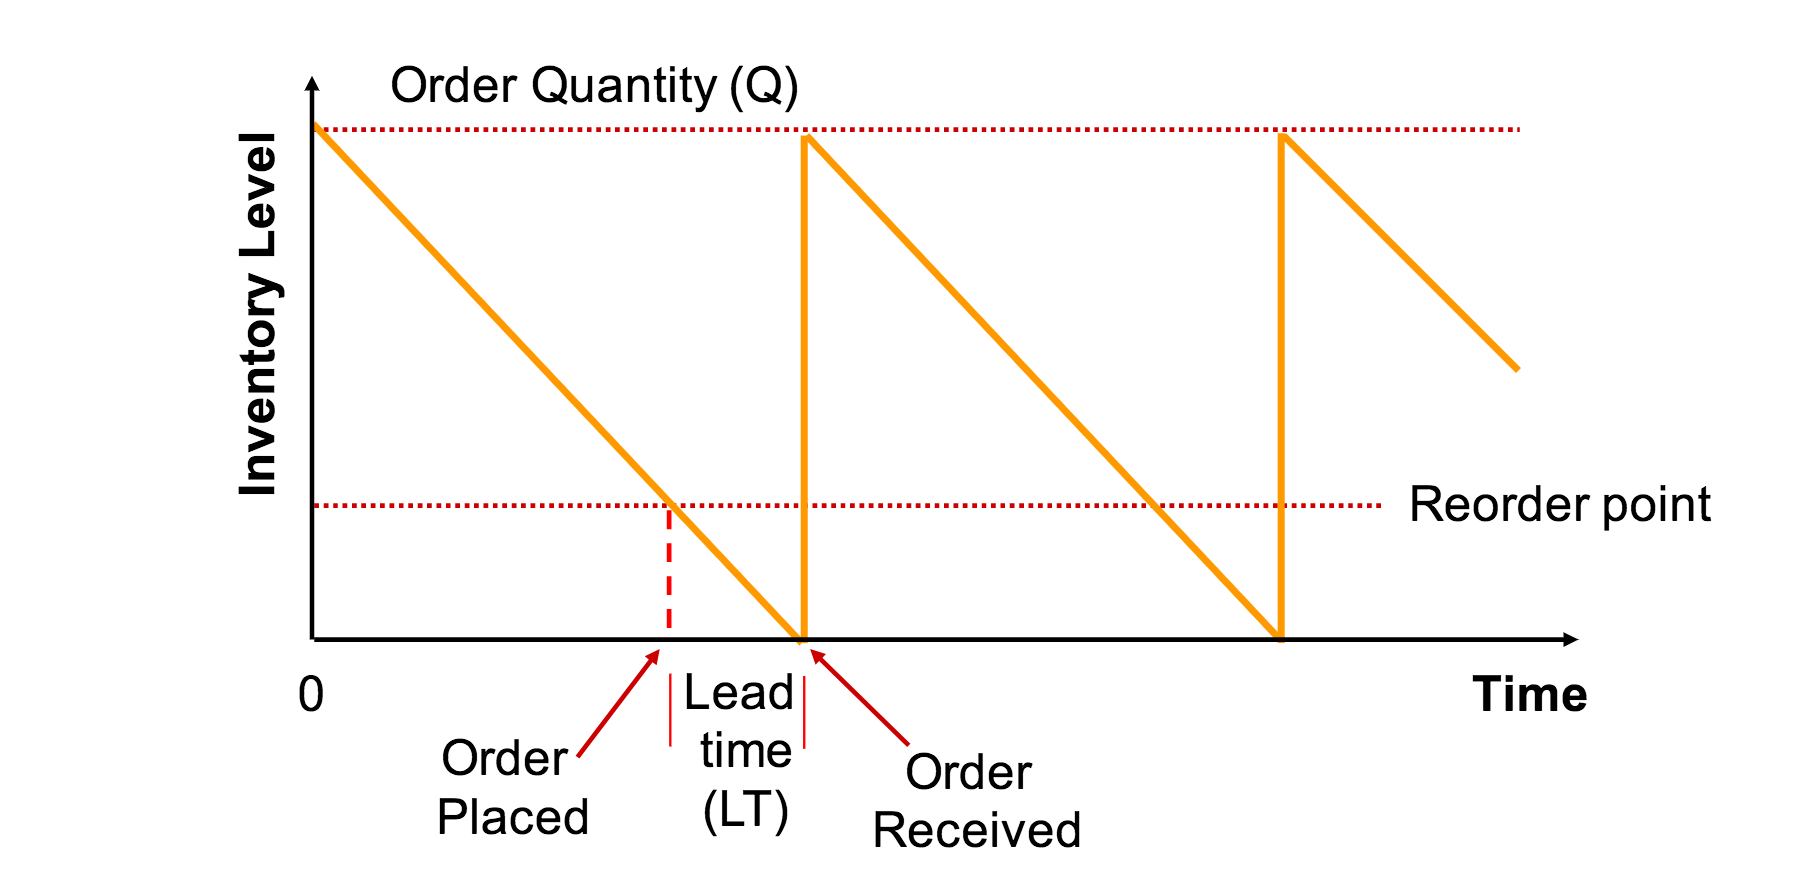
\includegraphics[width=0.5\textwidth]{sawtooth}
\end{figure}
The cost per period is given by\ix{Cost per Period}
\begin{align*}
T(Q) = \frac{Q}{2}C_h + \frac{D}{Q} C_O \Rightarrow \text{EOQ} = \sqrt{2D\frac{C_O}{C_H}}
\end{align*}
where $Q$ is the batch size, $D$ is the demand per period, $C_O$ is the order cost and $C_H$ is the holding cost. The Economic Order Quantity is determined by using the first order condition. Strictly speaking, the holding cost for safety stock and the variable cost per item should be included. 

Problems with this model is that the assumptions made are very rigid (e.g. many quantities are assumed to be constant). It also relies on getting good number of the holding and ordering costs. It is robust, tends to inflate order sizes. Empirically, $<12\%$ from the optimum. 

\item The Newsvendor Model applies under stochastic demand. \ix{Newsvendor Model}The demand CDF is required as are the overage/underage costs. 
\begin{align*}
G(Q,D) &= c_o \max(0, Q-D) + c_u \max(0, D-Q) \\
\frac{d}{dQ} \big ( \mathbb{E}_D[G(Q, D)]\big )&=0 \Rightarrow F_D(Q^*) = \frac{c_u}{c_o + c_u}
\end{align*}
and thus it is easily see that if $c_u = c_o$, $Q^*=\expt{D}$


\item\ix{(Q,R) Policy}This is an extension of the EOQ model but now both $Q$ and $R$ are decision variables and the cycle time is not constant. Demand is assumed to be random and stationary with a fixed lead time, $L$. Denote the holding cost as $C_H$, the setup cost per order $C_O$ and the penalty per unit of unsatisfied demand $p$. The expected demand per unit time is $\lambda$.


\begin{align*}
C(Q) = C_h(\underbrace{\frac{Q}{2} + R - \lambda L}_{\text{Average Stock}}) + \frac{C_O}{Q/\lambda} + p \frac{\expt{\max(0, D-R)}}{Q/\lambda}
\end{align*}
The first order conditions can be applied to $Q$ and $R$ leading to the following equations which must be solved iteratively
\begin{align*}
Q = \sqrt{\frac{2\lambda(C_O+ p n(R))}{C_H}} \hspace{1cm} F_D(R) = 1 - \frac{QC_H}{p\lambda}
\end{align*}
The final solution is a compromise between the shortage costs (large $R$), holding costs (small $Q$ and $R$) and the fixed costs. 

\item\ix{Decision Rules}There are the number of decisions rules which can be used:
\begin{itemize}
	\item \textbf{Minimax}: Maximise the absolute maximum possible payoff. Generally highly risky. 
	\item \textbf{Maximin}: Maximise the minimum possible payoff. Quite conservative. 
\end{itemize}

\item\ix{Decision Analysis: Definitions}Often it the probabilities of different states of nature can be determined. 
\begin{enumerate}
	\item The expected monetary value is the expected value of decision i
	\begin{align*}
		\text{EMV}_i = \sum_j r_{ij} p_j
	\end{align*}
	where $r_{i}$ is the payoff for decision $i$ under outcome $j$.
	
	\item The expected opportunity loss is the expected regret of decision $i$
	\begin{align*}
	g_{ij} = \underbrace{(\max_k r_{kj}) - r_{ij}}_{\text{Regret}} \hspace{1cm} \text{EOL}_i = \sum_j g_{ij} p_j =  \sum_j (\max_k r_{kj}) p_j  - \text{EMV}_i 
	\end{align*}
	i.e. the regret is the difference between the payoff of the decision chosen and the maximum payoff given an outcome. Thus, \textbf{the decision with the largest EMV has the minimum regret}.
	
	\item If the future could be predicted with $100\%$ accuracy, the strategy could be optimised. 
	\begin{align*}
	\text{PI} = \sum_j (\max_i r_{ij}) p_j 
	\end{align*}
	The expected value of perfect information is the difference between PI and the maximum EMV (which is the same as the minimum EOL).
	\begin{align*}
	\text{EVPI} = \text{PI} - \max_i (\text{EMV}_i ) = \min (\text{EOL}_i)
	\end{align*}
	
	\item If probabilities estimates can be refined, they add value. The \textbf{expected value of sample information} (EVSI) is the difference between the EMV with the same information and the EMV without. 
\end{enumerate}
These measures don't consider the spread of pay-offs, an issue remedied by utility theory. Replacing the pay-offs with the utility for a payoff is a solution to this (and the utility curve defines the risk preferences e.g. $\expt{U(X)} > U(\expt{X})$ describes risk seeking preferences).

\item \ix{Dynamic Programming}Dynamic programming is a technique used to solve complex problems by breaking them down into smaller problems and then solving using \emph{backwards induction}. The problem is defined as follows; note that a * denotes optimality.
\begin{itemize}
	\item $N$ is the number of stages.
	\item $n \in \lbrace 1, \ldots, N \rbrace$ is the stage index.
	\item $s_n$ is the state variable for stage n.
	\item $s_n$ is the decision variable for stage $n$.
	\item $s_{n+1} = g_n(s_n, x_n)$ i.e. $g(\cdot)$ represents the system transition between stages given a choice of the decision variable. 
	\item $c_n(s_n, x_n)$ represents the contribution to the system value in a given stage, $n$.
	\item $f_n(s_n, x_n)$ represents the \emph{total} contribution of all following stages if the state is $s_n$ and the decision taken is $x_n$ and optimal decisions are made subsequently. 
\end{itemize} 
Thus the Bellman optimality equation is formed\ix{Bellman Equation}
\begin{align*}
f^*_n(s_n) = \min_{x_n} (c_n(s_n, x_n) + f^*_{n+1}(g_n(s_n, x_n)))
\end{align*}
This technique finds use in stochastic situations where the transition function, $g(\cdot)$, is replaced by a probability mass function and the expectation is minimised (in the Bellman equation). 

\item\ix{Markov Chains}A few definitions for markov chains have been included below:
\begin{itemize}
	\item State $j$ is accessible from $i$ if there is a path from $i \rightarrow j$. If $i \leftrightarrow j$, $i\ \&\ j$ are said to communicate.
	\item A class, $A$, is absorbing if for each $i\in A$, $i\rightarrow j \Rightarrow j\in A$. Thus it is impossible to escape from an absorbing class. A state is absorbing if it is a absorbing class itself. 
	\item Class $B$ is accessible from class $A$ if $\forall i\in A\ \&\ \forall j\in B, i \rightarrow j$.
	\item A chain with a single class is irreducible. 
	\item A state is recurrent can be visited an infinite number of times. A transient state is only visited a finite number of times. 
	\item A state is aperiodic if $p_{ii}^(n) > 0$ for all sufficiently large $n$. Note that this is a class property. 
	\item A Markov chain is period with period $m$ if the process can only recur to state $i$ after $km$ steps. 
	\item If a Markov chain is irreducible and aperiodic then there is a limiting distribution.
	\item The invariant distribution is given by $\vect{\pi P = \pi}$; this is useful to calculate e.g. average payoff per unit time. 
\end{itemize} 
Note that, by the law of total probability,
\begin{align*}
p_{ij}^{(n)} = \sum_k p_{jj}^{(n-k)}f_{ij}(k)
\end{align*}
where $p_{ij}^{(n)}$ is the probability of ending in state $j$ after $n$ steps after starting in state $i$ and $f_{ij}(k)$ is the probability that the first passage from $i$ to $j$ occurs after $k$ transitions. This gives a recursive set of relations. This allows the expected first passage time to be calculated, $\sum_k k f_{ij}(k)$. Alternatively, a set of linear equations can be set up. 

\item\ix{Continuous Time Markov Chains}With continuous time Markov chains, the rates determine the density function of the waiting times:
\begin{align*}
f(t) = \lambda e^{-\lambda t}
\end{align*}
The probability of arriving in an interval is $\lambda \Delta t$. The exponential distribution shows the \emph{lack of memory property} as required. In order to find the steady state, consider the \emph{balance equations} and recall that the probabilities must sum to one. 

\item\ix{Queueing Notation}Simple queueing systems are labelled as $U/V/s/\kappa/W$ where
\begin{itemize}
	\item $U,\ V$ denote the inter-arrival and service time distributions. Can be $D \text{ deterministic}$, $M \text{ memoryless}$ or $G \text{ general}$.
	\item $s$ denotes the number of serves.
	\item  $\kappa$ is the system capacity.
	\item $W$ is the queueing protocol (e.g. FIFO). 
\end{itemize}
Define the utilization factor, $\rho = \frac{\lambda}{s \mu}$, which is the expected fraction of time the service is expected to be busy. We define the follow additional performance measures where $p_i$ is the probability of having $i$ customers:
\begin{enumerate}
	\item Expected number of customers, $L = \sum_i^\infty ip(i)$.
	\item Expected queue length of a system with $s$ servers, $L_q = \sum_i^\infty ip(i+s)$.
	\item Average queue waiting time, $W_q$.
	\item Average waiting time, $W = W_q + \frac{1}{\mu}$.
\end{enumerate}
Littles formula says that $L_q = \lambda W_q$ and  $L=\lambda W$ \textbf{at steady state} since the number of customers leaving the queue must also enter the queue in steady state. 

\item If $X_1, \ldots, X_n$ are i.i.d. according to the exponential distribution, the minimum is also exponentially distributed with parameter $\lambda = \sum_i \lambda_i$. When there are multiple customer types, the average inter-arrival time is taken to be the mean. 

\item\ix{Regression}We assume that $y = \alpha + \beta x + \epsilon$ and see to find parameters such that the deviations between model predictions and observations is small $\hat{y_i} = a + bx_i$. This is done by minimising the least squares error using the familiar first order conditions.
\begin{align*}
\text{ESS} = &\text{S} = \sum_i (y_i - \hat{y_i})^2  \Rightarrow b = \frac{S_{XY}}{S_{XX}} , a = \bar{y} - b \bar{x} \\
\text{where } &S_{XX}= \sum_i (x_i - \bar{x})^2 \hspace{1cm} S_{XY}=\sum_i (x_i - \bar{x})(y_i - \bar{y})
\end{align*}
There are also other forms of deviation including the total sum of squares, $\text{TSS} = \sum_i (y_i - \bar{y})^2$ which measures the variation in $y$ around the mean and the regression sum of squares, $\text{RSS} = \sum_i (\hat{y_i} - \bar{y})^2$. Note that $\text{TSS} = \text{ESS} + \text{RSS}$.

It is important to understand the summary statistics:
\begin{itemize}
	\item $R = \frac{S_{XY}}{\sqrt{S_{XX} S_{XY}}}$ is known as the \textbf{correlation coefficient} and is a measure of the strength of the relationship. Note that $b=R\sqrt{\frac{S_{YY}}{S_{XX}}}$.
	\item $R^2 = \frac{RSS}{TSS}$ (where the square is only valid for regression); the closer to 1, the better the estimated regression fits the data. There also exists an \emph{adjusted} $R^2$ statistic which accounts for the number of data points. 
	\item The standard error, $S_e = \sqrt{\frac{\sum_i (y_i - \hat{y_i})^2}{n-1}}$, measures the scatter in the data around the regression line. 
	\item A rule of thumb for approximating a $95\%$ prediction is $[\hat{y} - 2S_e, \hat{y} + 2S_e ]$. 
	\item Large values of the $t$-statistic and small values of the $p$-value indicate that a variable used is significant. The $p$-value represents the trail probability of the variable and is used with normal hypothesis testing. 
\end{itemize}
$a$ and $b$ are unbiased estimators which are in fact normally distributed which allows confidence values to be obtained. There is a problem of multicollinearity in multiple regression models if two variables used are highly correlated. Coefficient estimates may change dramatically when a variable is removed. This can give large $p$-values even if the variable used is significant. Note that the model can be easily extended to non-linear regression. 

\ix{Forecasting}The forecasting error is defined as the difference between actual and forecasted value. There are several measures of forecast accuracy including:
\begin{itemize}
	\item Mean absolute deviation, $\text{MAD} = \frac{1}{N} \sum_i |e_i|$.
	\item Mean squared error, $\text{MSE} = \frac{1}{N} \sum_i e_i^2$.
	\item Mean Absolute Percentage Error $\text{MAPE} = \sum_i |\frac{e_t}{X_t}\frac{100}{N}|$
\end{itemize}
There are many different forecasting methods:
\begin{enumerate}
	\item The Moving Average
	\begin{align*}
	F_{t+1} = \frac{X_t + \cdots X_{t-m+1}}{m}
	\end{align*}
	
	\item Holt-Winter's Multiplicative Smoothing (\textbf{Don't Learn - on the datasheet!})
	\begin{align*}
		E_t &= \alpha \frac{X_t}{S_{t-c}} + (1-\alpha)(E_{t-1} + T_{t-1}) \\
		T_{t} &= \beta(E_{t} - E_{t-1}) + (1-\beta)T_{t-1} \\ 
		S_t &= \gamma \frac{X_t}{E_{t}} + (1-\gamma)S_{t-c} \\
		F_{t+k} &= (E_t + kT_t)S_{t+k-c}
	\end{align*}
	 $c$ is the number of time periods per season. The parameters can be set to zero also to give simpler forms of smoothing e.g. $T=0$ gives exponential smoothing with seasonality. To initialise this method, a complete season of data is required to determine the initial estimates for $S_t$ (but it is better to have two seasons for the trend).
	 
	 \item Holt-Winter's Additive Smoothing
	 \begin{align*}
	 E_t &= \alpha (X_t - S_{t-c}) + (1-\alpha)(E_{t-1} + T_{t-1}) \\
	 T_{t} &= \beta(E_{t} - E_{t-1}) + (1-\beta)T_{t-1} \\ 
	 S_t &= \gamma (X_t - E_t) + (1-\gamma)S_{t-c} \\
	 F_{t+k} &= E_t + kT_t + S_{t+k-c}
	 \end{align*}
\end{enumerate}
In each case, the best values of the parameters can be found via optimisation. Suitable initialisations for the values include $E_0 = X_0$. Set $T_0$ to the average trend across a season and $S_{i-c} = \frac{X_{i-c}}{\sum_j^c X_{j-c}/c}$.

\item\ix{Portfolio Management}An investor choosing a portfolio, $(\alpha_1, \alpha_2, \ldots, \alpha_n)$ which are real numbers (thus assuming \textbf{divisibility, liquidity and allowing for shorted assets}). Define
\begin{itemize}
	\item Assume $A_i(t)$ is the wealth at time $t$ of the asset $i$.  The wealth is
	\begin{align*}
	V(t) = \sum_i \alpha_i A_i(t)
	\end{align*}
	\item The rate of return is
	\begin{align*}
	K_A = \frac{A(t)-A(0)}{A(0)}
	\end{align*}
	\item The portfolio can be expressed in weights. Thus the portfolio return is 
	\begin{align*}
	K_v = \sum_i \omega_i K_i \text{ where } \omega_i = \frac{\alpha_i A_i(0)}{V(0)}
	\end{align*}
\end{itemize}
	Note that the prices are stochastic; we seek to maximise the expectation of the rate of return. Risk is quantified using the standard deviation. It is possible to plot portfolios on a graph of mean and variance; investors will then choose the minimum variance portfolio for a given mean (or the largest mean for a given variance). A portfolio is efficient if there is no other portfolio which has a strictly higher return with a strictly lower variance. 

Many models treat portfolio selection as a constrained optimisation problem e.g. minimise the variance given a mean. These problems can be solved using many software packages. Note as the number of securities increases, the optimisation problem becomes harder. 

A risk-less asset has zero standard deviation.Any point on the line that connects a portfolio and the risk-less asset forms a new portfolio. In this case, any efficient portfolio can be expressed as a combination of $P$ and the risk-less asset. The \textbf{one-fund theorem} states that there is a single fund of risky assets $P$ that can be decomposed as a combination of the fund $P$ and the risk-free asset.  

In market equilibrium, it is assumed that everybody solves the same problem and thus every investor holds the \textbf{market portfolio}. The weight is equal to the proportion of that asset's total capital value over the total market cap. Thus the optimal portfolio is the market portfolio and we don't need to solve the problem. Equilibrium in the market will force the market into the direction that solves the mean-variance problem since the prices will change, thus changing the optimal portfolio. This is similar to supply and demand matching. 

The capital market line is the line with the highest slope amongst all lines connecting the risk-less asset to the curve (and the tangency point is the market portfolio). This dominates any portfolio on the original frontier and all portfolios on this line have the same incremental rate of return per unit risk.  Thus for any efficient portfolio:
\begin{align*}
r = r_f + \frac{r_M - r_F}{\sigma_M}\sigma
\end{align*}
The $\beta$ for an asset measures the risk that the security contributes to a portfolio. If the market portfolio $M$ is efficient then
\begin{align*}
r_i - r_f = \beta_i(R_m - r_f) \hspace{1cm} \beta_i = \frac{\sigma_{iM}}{\sigma_{M}^2}
\end{align*}
$r_i - r_f$ is the expected excess rate of return of the asset which is linked to the excess rate of return of the market portfolio with proportionality factor $\beta$. This can be obtained by applying simple regression analysis for returns of the asset and the market portfolio. The security market line plots the excess asset return against $\beta$; if an asset if above this line, it is undervalued and if below the line it is overvalued. 


\end{enumerate}
\end{document}